\documentclass[11pt]{article}

% ---------- Geometry & typography ----------
\usepackage[margin=1in]{geometry}
\usepackage{microtype}
\usepackage[T1]{fontenc}
\usepackage{lmodern}
\emergencystretch=3em

% ---------- Math ----------
\usepackage{amsmath}
\usepackage{amssymb}

% ---------- Tables and figures ----------
\usepackage{booktabs}
\usepackage{graphicx}
\usepackage{array}
\usepackage{tabularx}
\usepackage{multirow}
\usepackage[section]{placeins}

% ---------- References ----------
\usepackage[numbers,sort&compress]{natbib}
\usepackage{url}

% ---------- Links ----------
\usepackage[hidelinks]{hyperref}

% ---------- Verbatim ----------
\usepackage{verbatim}

% ---------- Convenience macros ----------
\newcolumntype{Y}{>{\raggedright\arraybackslash}X}
\makeatletter
\setlength{\@fptop}{0pt}
\setlength{\@fpsep}{12pt plus 2pt}
\setlength{\@fpbot}{0pt plus 1fil}
\makeatother
\setcounter{topnumber}{5}
\setcounter{bottomnumber}{5}
\setcounter{totalnumber}{8}
\renewcommand{\topfraction}{0.95}
\renewcommand{\bottomfraction}{0.85}
\renewcommand{\textfraction}{0.05}
\renewcommand{\floatpagefraction}{0.75}
\newcommand{\acc}[1]{\ensuremath{\mathrm{acc}(#1)}}
\newcommand{\ndid}{\ensuremath{\Delta\mathrm{DiD}}}
\newcommand{\cohenh}{\ensuremath{h}}
\newcommand{\NUM}{\textbf{[NUM]}}
\newcommand{\TODO}[1]{\textbf{[TODO: #1]}}

% Override the article-class abstract: by default it applies \small font
% AND a \quotation-style indent on both margins, which makes the abstract
% visually narrower and smaller than body text. We want it to match the
% introduction's typography exactly.
\makeatletter
\renewenvironment{abstract}{%
  \begin{center}{\bfseries\large\abstractname\vspace{-.5em}\vspace{\z@}}\end{center}%
  \par\noindent\ignorespaces%
}{%
  \par\bigskip%
}
\makeatother

\title{Reasoning Enablement as a Selective Intervention:\\
A Preregistered Within-Family Study of Multi-Turn Pathologies}

\author{Tanishq Padwal\\
\small Independent Researcher\\
\small \texttt{padwaltanishq@icloud.com}}

\date{\today}

\begin{document}

\maketitle

\begin{abstract}
Multi-turn pathologies in large language models---self-consistency drift,
context rot, and sycophancy---have each been documented in isolation.
What remains unclear is whether a model's \emph{reasoning-enabled}
variant changes these failures uniformly, or only on some axes. We test
this with a preregistered, paired study of four Chinese open-weight model
families: DeepSeek V4-pro, DeepSeek V4-flash, Qwen3-235B, and Qwen3-30B.
Each family contributes an instruct member and a reasoning member. The
DeepSeek pairs provide the cleanest contrast: the same underlying model,
served by the same upstream, toggled between reasoning on and reasoning
off at request time. The Qwen pairs match base family and active
parameter count, but their instruct and thinking SKUs use different
upstream providers, which we treat as a caveat throughout.

Hypotheses, primary metrics, effect-size thresholds, multiple-comparisons
correction, exclusion rules, and falsification criteria were locked before
real-model data collection. We measure three verifiable, integer-scored
tasks: hard arithmetic self-consistency, $20$-update variable tracking,
and arithmetic-with-pushback. Reasoning-enabled variants show large and
universal self-consistency advantages ($\Delta_{\mathrm{acc}}$ of
$+0.67$ to $+0.99$ across the four pairs, sign-test BH-$q < 10^{-11}$
in every family). Sycophancy is heterogeneous: V4-flash shows a clean
within-MODEL reasoning gain ($+0.165$, BH-$q \approx
5{\times}10^{-4}$), V4-pro is null at threshold ($+0.045$, CI
$[-0.06, +0.15]$), and Qwen shows larger but capability-confounded gains.
Context rot is the least clean axis: DeepSeek is ceiling-bound, while
Qwen shows a substantial reasoning advantage entangled with instruct-side
mode collapse. We interpret reasoning enablement as a \emph{selective}
intervention---reliably effective on hard single-shot inference,
heterogeneous on pushback resistance, and not a universal fix for
multi-turn state tracking.

\end{abstract}

\section{Introduction}
\label{sec:introduction}

Large language models that succeed on a single-turn benchmark routinely
fail when the same task is embedded in a longer interaction. Three
failure modes have attracted particular attention over the past year.
\emph{Self-consistency drift}: identical prompts at temperature zero
produce different answers across replays, even on closed-source endpoints
\citep{atil2024nondeterminism,he2024numerical,gat2025outputdrift}.
\emph{Context rot}: accuracy degrades as filler turns accumulate between
the relevant information and the probe, with the bulk of the loss
attributable to growing unreliability rather than capability loss
\citep{laban2025lostmulti,liu2025drift,ren2026intent}.
\emph{Sycophancy}: once a model has yielded to a user assertion, that
agreement-seeking behaviour persists across subsequent turns
\citep{hong2025sycon,fanous2025syceval,zhang2025sycopressure}. Each line
of work has built its own metric (Number of Flip, ToF, accuracy decay
slope), its own pressure protocol, and its own model panel.

What no published study has done is hold the model family fixed and ask
whether \emph{reasoning-enabled variants}---models in their thinking-on
mode, regardless of whether the underlying weights are separately
post-trained or merely served with a reasoning flag flipped---shift these
three pathologies in a coordinated way or in opposite directions. The
closest result is in SYCON Bench \citep{hong2025sycon}, which notes in
passing that reasoning-optimised models resist sycophancy better than
instruction-tuned ones on a heterogeneous panel; but that observation
crosses model families and mixes architectures, so the reasoning effect
is confounded with scale, data, and base model. No prior work runs a
paired, within-family comparison across multiple pathology axes at once,
and none locks the analysis plan before collecting data.

We deliberately avoid the stronger claim that this paper measures the
effect of separate reasoning-style post-training, because two of our
four pairs are not separately post-trained. DeepSeek V4-pro toggles
between instruct and reasoning behaviour at request time through a
provider-side flag on the \emph{same} underlying model. The cleaner
within-family-and-within-weights contrast lives on the DeepSeek pairs;
the Qwen contrast is matched only at the family-and-scale level, with the
SKUs served by different upstream providers. We make this distinction
explicit in the design (\S\ref{sec:method}) and weight conclusions
accordingly.

We close that gap. The contribution of this paper is a preregistered,
within-family, multi-axis comparison of reasoning and instruct variants
on the same task suite, with the same paired statistical test, on the
same task seeds. The four model pairs are drawn from the Chinese
open-weight ecosystem because that ecosystem ships explicit
instruct/reasoning siblings of the same family: DeepSeek V4-pro toggled
between instruct and reasoning modes via an OpenRouter routing parameter;
DeepSeek V4-flash toggled between the legacy \texttt{deepseek-chat} and
\texttt{deepseek-reasoner} aliases that share weights but differ in
serving-time reasoning behaviour; Qwen3-235B and Qwen3-30B, each shipped
as separate instruct and thinking SKUs at the same active-parameter
count. For each pair we run three experiments---hard arithmetic
self-consistency, $20$-update variable tracking under filler pressure,
and hardness-5 arithmetic with wrong, correct, and neutral
pushback---scored by deterministic integer extraction (no LLM judges).
Hypotheses, primary metrics, an effect-size floor of Cohen's $h \geq
0.20$, BH multiple-comparisons correction within each axis, six frozen
exclusion classes, and falsification criteria were committed in
\texttt{PREREGISTRATION.md} on 2026-05-13 and amended on a dated log
before real-model data collection.

The findings preview as follows. The headline pattern is that
reasoning-enabled variants do \emph{not} provide a uniform robustness
boost across the three axes. On \textbf{self-consistency} they show
large, consistent gains in every family ($\Delta_{\mathrm{acc}}$ of
$+0.67$ to $+0.99$, sign-test BH-$q < 10^{-11}$). On
\textbf{sycophancy} the pattern is heterogeneous within the family of
reasoning-enabled variants: V4-flash shows a clean within-MODEL effect
(reasoning-gain $+0.165$, BH-$q \approx 5{\times}10^{-4}$); V4-pro is
null at the preregistered $|\mathrm{gain}|\geq 0.10$ threshold (gain
$+0.045$, CI $[-0.06, +0.15]$); the Qwen pairs show larger gains that
are partially confounded with an instruct-side capability mode-collapse
on hard arithmetic. On \textbf{context rot} the DeepSeek pairs are
dominated by ceiling effects (instruct already at $1.000$ accuracy
across most cells, leaving no headroom), and the Qwen pairs show a
substantial reasoning advantage that is again partially entangled with
the same capability gap. We frame this as a \emph{selective}
intervention---reliably effective on hard single-shot inference,
heterogeneous on pushback resistance, and conferring no measurable
additional benefit on multi-turn state-tracking when the instruct
sibling is already at ceiling. The remainder of the paper
develops this in detail. Section~\ref{sec:related} positions the work
against the three axis-specific literatures; Section~\ref{sec:method}
explains the paired design and the four model pairs;
Section~\ref{sec:hypotheses} states the locked analysis plan;
Section~\ref{sec:setup} reports the exact sweep parameters and
exclusion accounting; Sections~\ref{sec:results}--\ref{sec:conclusion}
present results, discussion, and limitations.

\section{Related Work}
\label{sec:related}

We organise prior work by the three pathology axes we measure, then state
the precise gap our design addresses.

\paragraph{Context rot.}
\citet{laban2025lostmulti} ran more than $200{,}000$ simulated multi-turn
conversations across six task domains and reported an average $39\%$
accuracy drop relative to the equivalent single-turn problem, decomposable
into a small aptitude loss and a large unreliability increase.
\citet{liu2025drift} reframe the phenomenon as a context-equilibrium
problem, and \citet{ren2026intent} attribute the drop primarily to
turn-by-turn intent mismatch. \citet{zhao2026conversationtree} introduce
the related notion of ``logical context poisoning'' from progressive
structural corruption. Adjacent but distinct lines include
single-prompt long-context benchmarks such as NOLIMA
\citep{modarressi2025nolima} and memory-architecture evaluations such as
MemoryAgentBench \citep{hu2025memoryagentbench}.

\paragraph{Sycophancy.}
\citet{hong2025sycon} introduce SYCON Bench with \emph{Turn-of-Flip} and
\emph{Number-of-Flip} metrics for multi-turn sycophancy and report---on a
heterogeneous panel that crosses families---that reasoning-optimised
models generally resist sycophancy better than instruction-tuned models.
\citet{fanous2025syceval} report that ``once a model yields to a user
assertion, agreement-seeking behaviour often persists across subsequent
turns'', the verbatim phrasing of the persistence claim. Domain
variations cover scientific QA \citep{zhang2025sycopressure}, clinical
encounters \citep{kim2026sycoevalem}, financial agents
\citep{wang2026priceofagreement}, and moral-judgment perturbations
\citep{li2026moralfragility}. \citet{xu2025notonething} argue
sycophancy is causally decomposable rather than monolithic, and
\citet{chen2025beacon} propose a single-turn diagnostic for latent
sycophantic tendencies.

\paragraph{Self-consistency under deterministic settings.}
\citet{atil2024nondeterminism} report up to $15\%$ accuracy variance and
a $70\%$ best-to-worst gap across $10$ replays of the same prompt under
nominally deterministic configuration. \citet{he2024numerical} give a
mechanistic explanation: tiny logit gaps combined with BF16/FP16
numerical fluctuations cause non-determinism that disappears under FP32.
\citet{shen2025smallllmnondet} extend this to $2$--$8$B models, and
\citet{gat2025outputdrift} document the cross-provider variant in which
the same model name returns different distributions across hosting
providers.

\paragraph{Agent-failure context.}
\citet{wang2025agentfail}, \citet{yu2025trajectbench}, and
\citet{lin2025agentracer} build failure taxonomies and localisation
methods for tool-using agents. These are adjacent neighbours rather than
direct competitors: our setting is multi-turn conversational
pathologies, not tool execution.

\paragraph{What is novel here.}
Each of the works above studies one pathology axis on its own panel and
in many cases on a single model family. Where reasoning-enabled variants
are implicated---most explicitly in SYCON \citep{hong2025sycon}---the
comparison crosses model families, so the reasoning-mode effect is
confounded with base architecture and scale. To our knowledge, this is the first
study that simultaneously (i) applies a within-family paired design
across multiple model families, (ii) measures three pathology axes on
the same pairs with the same task seeds, and (iii) preregisters
hypotheses, effect-size floors, multiple-comparisons correction, and
exclusion rules before any real-model data was collected.

\paragraph{Design-strength caveat by family.}
Within the within-family-paired framing, our four pairs are \emph{not}
controlled to the same degree, and we are explicit about which contrast
each pair supports. The DeepSeek V4-pro and V4-flash pairs are the
strongest contrast: in each, the same underlying model is served by the
same upstream provider, with the reasoning behaviour toggled at request
time---so base weights, scale, and serving host are all held fixed and
the only varying factor is the runtime reasoning flag (V4-pro) or the
model-alias selection that maps to the same weights with thinking on/off
(V4-flash). The Qwen3-235B and Qwen3-30B pairs are weaker: they match
base family and active-parameter count, but the instruct SKU and
thinking SKU are shipped as separate model identifiers and, in our
deployment, are served by \emph{different} upstream providers (Novita
vs Alibaba for Qwen3-235B; Nebius vs AtlasCloud for Qwen3-30B). We
treat the Qwen pairs as evidence of family-and-scale-matched
behavioural differences, but not as a same-weights-same-host contrast.
This soft caveat is reiterated wherever the Qwen pairs are discussed in
results.

\section{Methodology}
\label{sec:method}

The design decision that organises everything else is the within-family
pairing. We describe the pairing first
(\S\ref{sec:method:pairing}), then the three tasks
(\S\ref{sec:method:tasks}), and finally the operational guarantees that
make the pairing meaningful---upstream-provider pinning, frozen
exclusion classes, resumable execution, and verifiable scoring
(\S\ref{sec:method:ops}).

\subsection{Within-family paired design}
\label{sec:method:pairing}

A canonical comparison such as ``does enabling a model's reasoning mode
change multi-turn behaviour?'' is usually answered by reading off
accuracy deltas across heterogeneous panels---e.g.\ a reasoning-enabled
model from lab A against an instruct model from lab B. Such a comparison
conflates the reasoning-mode contrast with base model, scale, data mix,
RLHF recipe, and serving stack. We avoid that confound by restricting attention to four
model \emph{families} that ship matched instruct and reasoning siblings:

\begin{enumerate}
  \item \textbf{DeepSeek V4-pro.} Same weights, two
        configurations of the reasoning toggle. The original sweep
        was pinned to Novita via OpenRouter
        (\texttt{reasoning: \{enabled: false\}} for instruct,
        \texttt{reasoning: \{effort: "high"\}} for reasoning); per the
        2026-05-15 amendment a subset of cells was recovered via the
        DeepSeek first-party API with the V4-family-native
        \texttt{thinking: \{type: "enabled"\|"disabled"\}} parameter.
        The final analyzable dataset therefore mixes OR/Novita
        originals with DS-direct recoveries on a per-cell basis; see
        \S\ref{sec:methods:v4pro-routing} for the rationale, accounting,
        and per-axis breakdown.
  \item \textbf{DeepSeek V4-flash.} Same weights, served by DeepSeek
        direct. The legacy aliases \texttt{deepseek-chat} and
        \texttt{deepseek-reasoner} route the same family through the
        instruct and reasoning code paths respectively.
  \item \textbf{Qwen3-235B (a22b).} Two SKUs published by Alibaba at the
        same active-parameter count: \texttt{qwen3-235b-a22b-2507}
        (instruct, served via Novita) and
        \texttt{qwen3-235b-a22b-thinking-2507} (reasoning, served via
        Alibaba).
  \item \textbf{Qwen3-30B (a3b).} \texttt{qwen3-30b-a3b-instruct-2507}
        (served via Nebius) and \texttt{qwen3-30b-a3b-thinking-2507}
        (served via AtlasCloud).
\end{enumerate}

For DeepSeek pairs base architecture, scale, training run, and serving
host are all held constant; only the reasoning toggle varies, so the
paired contrast isolates the reasoning effect. For Qwen pairs the
families and active-parameter counts match, but the default upstream
host differs across siblings (Novita vs.\ Alibaba on the 235B pair;
Nebius vs.\ AtlasCloud on the 30B pair). We document this as a soft
limitation of the Qwen pairing's serving-stack equivalence
(\S\ref{sec:limitations}) and report Qwen and DeepSeek results
separately so a reader can attribute any disagreement to the routing
difference.

This design is stronger than the pairing proposed in the original
preregistration (\texttt{deepseek-v4-pro} vs.\ \texttt{deepseek-r1-0528}),
which crossed two distinct base models. The amendment log dated
\textsl{2026-05-13 (further)} replaces that exploratory pairing with the
within-model reasoning-toggle design above, eliminating the
architecture/scale confound on the DeepSeek side.

\subsection{Three tasks, all integer-scored}
\label{sec:method:tasks}

All tasks emit a single integer answer that is extracted from the
model's response by a strict regular-expression scorer with
word-boundary matching. No LLM judge is invoked at any point in the
analysis loop.

\paragraph{Self-consistency: hard arithmetic (hardness $5$).}
The model is asked to evaluate a closed-form arithmetic expression in
$12$ four-digit operands with squares, modulo, integer division, and
nested grouping. Hardness $5$ was chosen so frontier models do not
saturate at $100\%$---which would leave no headroom for either
divergence or accuracy measurement. The same task seed is replayed
$N{=}25$ times at temperature $0$ with the API seed fixed at the
\texttt{task\_seed}, so any cross-replay divergence is attributable to
serving-stack non-determinism rather than nominal sampling randomness.
Per-task divergence is the fraction of replays whose extracted answer
differs from the modal extracted answer.

\paragraph{Context rot: variable tracking ($n_{\mathrm{updates}} = 20$).}
The model maintains a running integer state \texttt{x} across $20$
chained update turns---each turn applies an add, subtract, or multiply
operation---then is asked at probe for the final value of \texttt{x}.
This is a stronger context-rot signal than single-fact recall because
the probe is unanswerable without actually carrying state across turns.
Between the update block and the probe we insert $n_{\mathrm{filler}}
\in \{0, 2, 5, 10, 20, 40\}$ filler turn-pairs of one of four kinds:
\texttt{irrelevant} (chitchat), \texttt{related} (math-adjacent),
\texttt{token\_matched} (fixed-length filler at the same turn count
controlling for content variability), and \texttt{collapsed} (a single
fat user-assistant pair whose total token mass matches the cumulative
token mass of $n_{\mathrm{filler}}$ small pairs). The
\texttt{collapsed} kind is the true turn-vs-token control: comparing
accuracy at (\texttt{irrelevant}, $k{=}20$) against (\texttt{collapsed},
$k{=}20$) holds total tokens approximately constant while collapsing
$40$ turns into $2$, isolating turn-count effects from token-mass
effects.

\paragraph{Sycophancy: arithmetic-with-pushback (hardness $5$).}
The protocol is original probe $\rightarrow$ model answer $A$
$\rightarrow$ user pushback $\rightarrow$ model answer $A'$ $\rightarrow$
$g$ neutral filler pairs $\rightarrow$ re-probe $\rightarrow$ model
answer $A''$ (scored). The pushback condition is one of three: in the
\texttt{wrong} condition the user asserts a wrong integer answer (a
$+7$ perturbation of the truth that preserves magnitude and sign); in
the \texttt{correct} condition the user asserts the right answer; in
the \texttt{neutral} condition the user expresses doubt without
asserting any value. The \texttt{correct} condition is the critical
control: a model that flips on \texttt{correct} pushback is generically
capitulating, not sycophantic. The interpretable signal is
$\acc{\mathrm{correct}} - \acc{\mathrm{wrong}}$. The post-pushback gap
is $g \in \{0, 2, 5, 10\}$ neutral filler pairs.

The 2026-05-14 amendment log records the switch from a CRT-style
counterintuitive-math task to hardness-5 arithmetic. The reason was
empirical: stage-1 calibration showed that reasoning models solved CRT
items so reliably at baseline that wrong pushback produced essentially
no flip rate---a ceiling that hid any reasoning-vs-instruct difference.
Hardness-5 arithmetic creates legitimate uncertainty in model answers,
giving wrong pushback room to register.

\subsection{Operational guarantees}
\label{sec:method:ops}

\paragraph{Upstream-provider pinning.}
Every OpenRouter request specifies a single pinned upstream host
(\texttt{configs/models.yaml: upstream\_provider}) with
\texttt{allow\_fallbacks: false}. Without pinning, OpenRouter
load-balances across upstream hosts---which would silently confound a
paired test if one sibling was served by a different actual provider on
different days. After each completion we verify the response's reported
provider header against the pinned value and tag a mismatch as a
distinct exclusion class
(\texttt{upstream\_provider\_mismatch}).

\paragraph{Six frozen exclusion classes.}
Trajectories are excluded from analysis if and only if they fall into
one of six classes, all frozen alongside the preregistration:
(i) \texttt{provider\_error:*}: the request never reached the model
after retries (HTTP failure or credit exhaustion). Because the model
never produced output, these are re-attempted on resume rather than
counted as model-behaviour exclusions.
(ii) \texttt{refusal\_detected}: detected by absence of any digit in
the probe answer for arithmetic and variable-tracking tasks.
(iii) \texttt{truncated\_at\_max\_tokens}: missing terminating
punctuation \emph{and} output length equal to \texttt{max\_tokens}.
(iv) \texttt{upstream\_provider\_mismatch}: a fallback fired despite
\texttt{allow\_fallbacks: false}.
(v) \texttt{empty\_probe\_answer}: scorer found no integer in a
non-empty response (a true scoring failure).
(vi) \texttt{provider\_empty\_response}: the provider returned HTTP $200$
with an empty body and \texttt{output\_tokens == 0}, added in the
2026-05-14 amendment after stage-1 calibration revealed
${\sim}1{,}100$ such rows misclassified as \texttt{empty\_probe\_answer},
concentrated on \texttt{deepseek-reasoner} and \texttt{deepseek-v4-pro
reasoning} via Novita.

\emph{Originally we treated these as deterministic and not silently
re-attempted; the 2026-05-15 amendment retracts that judgment.}
Targeted diagnostics on 2026-05-15 showed the empties were the
downstream consequence of our \texttt{max\_tokens}{=}2048 setting being
below the DeepSeek-recommended default of $32{,}000$ for reasoning
models, so the entire budget was consumed by \texttt{reasoning\_content}
(CoT) and \texttt{content} came back empty. Affected cells were re-attempted
through DeepSeek's first-party API with
$\mathrm{max\_tokens}\in\{8{,}192, 16{,}384\}$ and recovered cleanly;
the analyzable dataset is composed of the recovered rows via semantic
dedup (\S\ref{sec:methods:dedup}). The original $2048$-token rows
survive in the JSONL audit trail. Classes (ii)--(vi) remain reported
on whatever residual fraction the recovery did not clear; only (i)
\texttt{provider\_error} continues to be silently re-attempted under
the runner's resume logic.

\paragraph{Resumable runner with content-hashed cell keys.}
Each trajectory is keyed by a content hash of (model, task seed,
sweep-cell coordinates). The JSONL log is appended in place. On resume
the runner skips any cell whose key already exists in the log. This
guarantees that a transient infrastructure failure mid-sweep cannot
silently corrupt a cell---the missing rows are simply re-attempted on
the next run, and only rows that produced a real model response are
counted.

\paragraph{Verifiable scoring, no LLM judges.}
All three tasks score a single extracted integer against a known
ground-truth integer using word-boundary regular expressions
(\texttt{src/agent\_pathologies/tasks/scoring.py}). This avoids the
known reliability issues with LLM-judge scoring on arithmetic-adjacent
tasks and makes the entire analysis pipeline reproducible from the raw
JSONL.

\paragraph{Paired by task seed.}
The paired statistical tests in Section~\ref{sec:hypotheses} are
constructed by matching trajectories on
$(\mathrm{family}, \mathrm{task\_seed}, \mathrm{sweep\_cell})$. The same
seed is run on both members of a pair, so the comparison conditions on
task identity and not just on marginal accuracy.

\section{Hypotheses and Locked Analysis Plan}
\label{sec:hypotheses}

This section is reproduced from \texttt{PREREGISTRATION.md} (root) and
the per-experiment preregistrations, with the dated amendments folded
in. All content here was locked before any real-model data was
collected. The amendment log in the repository records every change to
this section with a date and reason.

\subsection{Hypothesis pairs}

For each pathology axis and each within-family pair we test a two-sided
hypothesis pair. Two-sidedness is intentional and strict: we report any
significant effect in either direction with equal seriousness, and we
do not claim a preregistered direction anywhere in the analysis plan.
This was a deliberate methodological choice---the literature contains
support for both possibilities (reasoning-enabled variants being more
robust on some axes; extended reasoning traces causing over-thinking
failures on others), and we elected not to bias the test or the
reporting in advance.

\begin{itemize}
  \item \textbf{Self-consistency.} $H_0$: within a family, instruct and
        reasoning siblings have the same answer-divergence distribution
        across $25$ replays of the same task at $T{=}0$. $H_1$: the
        distributions differ.
  \item \textbf{Context rot.} $H_0$: within a family, instruct and
        reasoning siblings have the same accuracy on the running
        variable-tracking task across the
        $(n_{\mathrm{filler}} \times \mathrm{kind})$ sweep. $H_1$: they
        differ---reasoning shifts the slope or intercept of the decay
        curve.
  \item \textbf{Sycophancy.} $H_0$: within a family, instruct and
        reasoning siblings have the same accuracy at re-probe after
        pushback across the $(\mathrm{condition} \times g)$ sweep.
        $H_1$: they differ.
\end{itemize}

\subsection{Paired statistical tests}

\paragraph{Self-consistency.} Per-task divergence is computed on the
\emph{extracted scored quantity} (not the raw response string), following
the 2026-05-14 amendment that found chain-of-thought verbosity inflated
string-level divergence well above answer-level divergence on stage-1
calibration data. The primary test is a paired Wilcoxon signed-rank on
per-task divergence across the $40$ tasks per family. A co-primary
paired Wilcoxon on per-task accuracy is added, because at hardness $5$ a
model can be highly \emph{consistent} while being highly
\emph{incorrect}---e.g.\ Qwen instruct emitted the same stock string to
${\sim}65\%$ of hardness-$5$ prompts during calibration. A family is
reported as positive only if at least one of the two paired Wilcoxon
tests crosses BH-corrected $q < 0.05$. Because the tests are two-sided,
the direction of the delta is reported but not used as a pass/fail
criterion.

\paragraph{Context rot.} Paired McNemar's exact test on
\texttt{is\_correct} per
$(\mathrm{family} \times \mathrm{kind} \times n_{\mathrm{filler}})$
cell, with Cohen's $h$ for the paired-proportion effect size and BH
correction across all $24$ cells within each family.

\paragraph{Sycophancy.} Two co-primary tests, both required to clear
their thresholds before a family is called positive.
(a) Paired McNemar's exact on \texttt{is\_correct} per
$(\mathrm{family} \times \mathrm{condition} \times g)$ cell, with
Cohen's $h$ and BH correction. (b) Between-model paired
difference-in-differences (DiD): for each $(\mathrm{family}, g)$ cell,
$\ndid = \big[\mathrm{reasoning}(\acc{\mathrm{correct}} -
\acc{\mathrm{wrong}})\big] - \big[\mathrm{instruct}(\acc{\mathrm{correct}}
- \acc{\mathrm{wrong}})\big]$, paired by task identity, with bootstrap
$95\%$ CI from $10{,}000$ resamples
(\texttt{paired\_did\_bootstrap}). The DiD is the cleaner statistical
expression of the research question and is reported as the headline
statistic; the McNemar is retained for cell-wise diagnostics. The
amendment dated 2026-05-13 promoted the DiD to co-primary.

\subsection{Effect-size thresholds}

Across all axes we require Cohen's $h \geq 0.20$ on paired proportions
to call a result substantive. For the sycophancy DiD we additionally
require $|\ndid| \geq 0.10$ on the proportion scale---a $10$ percentage
point gap in the differential responsiveness to wrong-versus-correct
pushback between siblings. Below these thresholds, a result is reported
as a null finding even if $p < 0.05$. Publication of null is fine; we
report it.

\subsection{Multiple-comparisons correction}

Within each axis, $p$-values are corrected with Benjamini--Hochberg at
target FDR $= 0.05$. Correction is applied across all pair-by-cell
tests within an axis but not across axes, because the three axes test
different operational hypotheses.

\subsection{Sample sizes and stopping}

\begin{itemize}
  \item Self-consistency: $N = 40$ tasks $\times 25$ replays per model.
  \item Context rot: $N = 50$ task instances $\times 6$ filler counts
        $\times 4$ filler kinds $\times 2$ roles $= 2{,}400$
        trajectories per family.
  \item Sycophancy: $N = 50$ task instances $\times 3$ pushback
        conditions $\times 4$ gaps $\times 2$ roles $= 1{,}200$
        trajectories per family.
\end{itemize}
All three are powered to detect $h = 0.25$ at $\alpha = 0.05$ with
$\geq 80\%$ paired-design power, assuming an intra-pair correlation of
$0.4$. No optional stopping: the full $N$ is run before any analysis.

\subsection{Falsification criteria}

The headline claim of the paper is that reasoning-enabled variants
systematically alter multi-turn pathology resistance within a family. The
preregistration commits us to report a null result---rather than
post-hoc reframing as a survey---under the following condition: if
McNemar/Wilcoxon returns BH-corrected $q > 0.05$ for \emph{all} four
families and $|h| < 0.20$ (and $|\ndid| < 0.10$ for sycophancy) for
\emph{all} cells, on \emph{all three} axes, then we conclude that
reasoning enablement does not systematically alter multi-turn pathology
resistance in these families. We also report axis-level null findings
even when other axes are positive, rather than burying or downplaying
them in the discussion. Any post-hoc reframing would itself be an
amendment, dated, and would require a fresh sweep.

\section{Experimental Setup}
\label{sec:setup}

This section reports the exact model identifiers, hyperparameters,
sweep dimensions, and exclusion accounting used to generate the
results.

\subsection{Models and upstream pinning}

Table~\ref{tab:models} lists the four within-family pairs with their
OpenRouter (or DeepSeek-direct) model identifiers, the pinned upstream
host, and the routing parameter that distinguishes the instruct member
from the reasoning member.

\begin{table}[h]
\centering
\small
\begin{tabularx}{\textwidth}{l l l l X}
\toprule
Family & Role & Model identifier & Upstream & Distinguishing parameter \\
\midrule
\multirow{2}{*}{\texttt{deepseek-v4-pro}$^\dagger$}
  & instruct  & \texttt{deepseek-v4-pro}\,/\,\texttt{deepseek/deepseek-v4-pro} & DS-direct\,/\,Novita & \texttt{thinking: \{type: "disabled"\}} (DS), \texttt{reasoning: \{enabled: false\}} (OR) \\
  & reasoning & \texttt{deepseek-v4-pro}\,/\,\texttt{deepseek/deepseek-v4-pro} & DS-direct\,/\,Novita & \texttt{thinking: \{type: "enabled"\}} (DS), \texttt{reasoning: \{effort: "high"\}} (OR) \\
\midrule
\multirow{2}{*}{\texttt{deepseek-v4-flash}}
  & instruct  & \texttt{deepseek-chat}     & DeepSeek direct & (instruct alias) \\
  & reasoning & \texttt{deepseek-reasoner} & DeepSeek direct & (reasoning alias) \\
\midrule
\multirow{2}{*}{\texttt{qwen3-235b}}
  & instruct  & \texttt{qwen/qwen3-235b-a22b-2507}          & Novita  & instruct SKU \\
  & reasoning & \texttt{qwen/qwen3-235b-a22b-thinking-2507} & Alibaba & thinking SKU \\
\midrule
\multirow{2}{*}{\texttt{qwen3-30b}}
  & instruct  & \texttt{qwen/qwen3-30b-a3b-instruct-2507} & Nebius     & instruct SKU \\
  & reasoning & \texttt{qwen/qwen3-30b-a3b-thinking-2507} & AtlasCloud & thinking SKU \\
\midrule
anchor (no pair) & instruct & \texttt{anthropic/claude-opus-4.7} & Anthropic & reported separately \\
\bottomrule
\end{tabularx}
\caption{Within-family pairs and upstream pinning. All OpenRouter
requests use \texttt{allow\_fallbacks: false}. Within each Qwen pair the
default upstream host differs across siblings (a soft serving-stack
limitation; see \S\ref{sec:limitations}). $^\dagger$ The
\texttt{deepseek-v4-pro} pair was originally pinned to OpenRouter via
Novita; per the 2026-05-15 PREREGISTRATION amendment, cells that
returned \texttt{provider\_error} or \texttt{empty\_probe\_answer} on
OR were re-attempted through DeepSeek's first-party API. The final
analyzable dataset is therefore \emph{mixed}: OR/Novita originals
that succeeded plus DS-direct recoveries for cells that the originals
did not produce. The slash-separated values list both
configurations; see \S\ref{sec:methods:v4pro-routing} for the per-axis
breakdown of the final mix.}
\label{tab:models}
\end{table}

\subsection{V4-pro routing amendment}
\label{sec:methods:v4pro-routing}

The \texttt{deepseek-v4-pro} pair was originally pinned to OpenRouter
via Novita, matching the upstream-pinning protocol applied to the other
OR-served families. Three independent observations on 2026-05-15
motivated a routing change to DeepSeek's first-party API
(\texttt{api.deepseek.com}) for all V4-pro retries:
(i)~\textbf{empty-response rate.}\ On long sycophancy and context-rot
conversations the OR-served V4-pro reasoning member returned a large
fraction of HTTP 200 responses with zero completion tokens, which our
runner correctly recorded as
\texttt{provider\_empty\_response} exclusions. Live testing against
\texttt{api.deepseek.com} with the documented native parameter
(\texttt{thinking: \{type: "enabled"\}}) and a budget of $16{,}384$
tokens reproducibly returned a populated \texttt{content} field on the
same prompts. (ii)~\textbf{the V4-family-native parameter is not
honoured for the legacy \texttt{reasoning} keyword.}\ The DeepSeek
documentation states explicitly that the V4 family uses
\texttt{thinking: \{type: "enabled"\|"disabled"\}}; the legacy
\texttt{reasoning: \{enabled: bool\}} is silently ignored. Empirically
we verified this on a controlled prompt: V4-pro responses with
\texttt{reasoning: \{enabled: false\}} continued to emit non-zero
reasoning tokens, whereas \texttt{thinking: \{type: "disabled"\}}
produced reasoning tokens of zero. (iii)~\textbf{methodological
parity}: V4-flash already used DeepSeek-direct, so routing V4-pro the
same way places both V4-family pairs on the model creator's API and
removes a confound between the two pairs. The 75\% promotional
discount on V4-pro through 2026-05-31 made the routing change financially
no worse than continuing on OR.

The retry rows written through DeepSeek-direct supersede the
\texttt{provider\_error} / \texttt{provider\_empty\_response} originals
via the semantic dedup at analysis time
(\S\ref{sec:methods:dedup}). Both rows remain in the raw JSONL
audit trail; the analyzable set picked by
\texttt{dedupe\_to\_latest} is composed of OR/Novita originals where
they succeeded, plus DS-direct retries on cells where the OR-served
original failed. Concretely (counts after dedup): on self-consistency,
$820$ of $1{,}000$ V4-pro-instruct and $400$ of $1{,}000$ V4-pro-reasoning
cells are OR-original; $180$ and $600$ respectively are DS-direct
recoveries. On sycophancy, $600$ of $600$ V4-pro-instruct cells are
OR-original; $260$ of $600$ V4-pro-reasoning are OR-original and the
other $340$ are DS-direct recoveries. On context-rot, the mix is
strongly OR-original: $1{,}187$ of $1{,}200$ V4-pro-instruct and
$1{,}168$ of $1{,}200$ V4-pro-reasoning come from the original Novita
sweep; the small DS-direct contributions ($13$ and $32$) are
recoveries on the cells where Novita returned errors or empty bodies.
The mix is heaviest on the reasoning sycophancy cells precisely
because that was the cell type most affected by the
\texttt{max\_tokens}{=}2048 bug.

\subsection{Hyperparameters per experiment}

Table~\ref{tab:hparams} reports temperature, max-tokens, sweep
dimensions, and total trajectories per family for each of the three
experiments. Temperature is fixed at $0$ on every call; the API seed is
held at the task seed for the self-consistency replays so that
remaining variance is attributable to serving-stack non-determinism.
The initial sweep used a \texttt{max\_tokens} budget of $2048$, which
turned out to be below the DeepSeek-recommended default of $32{,}000$ for
the \texttt{deepseek-reasoner} alias and caused systematic
empty-content responses on reasoning calls whose CoT exhausted the
budget. Per the 2026-05-15 PREREGISTRATION amendment, all retries on
DeepSeek reasoning cells used $\mathrm{max\_tokens}{=}8{,}192$ for
self-consistency / sycophancy and $\mathrm{max\_tokens}{=}16{,}384$ for
context-rot (whose longer input conversations leave less of the
\texttt{completion\_tokens} budget for content after reasoning); Qwen
instruct retries used $8{,}192$ to fix a smaller truncation issue on
$h{=}5$ arithmetic. The final analyzable dataset is composed of the
highest-token successful attempt per logical cell via the semantic
dedup (\S\ref{sec:methods:dedup}). The original $2048$ rows survive in
the JSONL audit trail.

\begin{table}[h]
\centering
\small
\begin{tabular}{l l l l l}
\toprule
Experiment & Task & Sweep dimensions & Per-pair $N$ & Hyperparameters \\
\midrule
self-consistency
  & arithmetic ($h{=}5$)
  & $40$ tasks $\times 25$ replays
  & $2{,}000$
  & $T{=}0$, max tok $2048$ \\
context rot
  & variable\_tracking ($n{=}20$)
  & $50 \times 6 \times 4$
  & $2{,}400$
  & $T{=}0$, max tok $2048$ \\
sycophancy
  & arithmetic ($h{=}5$)
  & $50 \times 3 \times 4$
  & $1{,}200$
  & $T{=}0$, max tok $2048$ \\
\bottomrule
\end{tabular}
\caption{Hyperparameters and sweep dimensions per experiment.
Per-pair $N$ counts trajectories collected on \emph{both} members of
the pair, so an effective paired sample size is half of this when
matched by task seed.}
\label{tab:hparams}
\end{table}

\subsection{Exclusion-rule definitions}

The six exclusion classes (\S\ref{sec:method:ops}) are defined formally
in \texttt{src/agent\_pathologies/analysis/exclusions.py} and applied at
analyzer read-time. Class~(i), \texttt{provider\_error}, is
infrastructure-only and re-attempted on resume; classes~(ii)--(vi) are
model-behaviour or serving-stack exclusions and are reported as-is.
Legacy rows tagged \texttt{empty\_probe\_answer} prior to the
2026-05-14 amendment are retroactively reclassified by
\texttt{metrics.py::reclassify\_legacy\_exclusions} based on the
\texttt{output\_tokens} field, idempotently.

\subsection{Semantic deduplication}
\label{sec:methods:dedup}

The raw JSONL is append-only: every retry attempt writes a new row,
even when retrying the same logical (model-family, role, task,
sweep-cell, seed) cell. For the analyzable dataset we apply
\texttt{dedupe\_to\_latest} (\texttt{src/agent\_pathologies/analysis/metrics.py}),
which keys cells on \emph{(model-family, role, task, sweep, seed)} —
intentionally broader than the runner's resume-key, which additionally
distinguishes by the raw model identifier. This broader key collapses
rows of the same logical cell that were served by different providers
(notably V4-pro originally via OR/Novita and re-served via
DeepSeek-direct in the retries), preferring any non-excluded row over
any excluded row, and tie-breaking on the latest non-excluded row. The
result is exactly one row per logical cell in the analyzed dataset
($N_{\mathrm{analyzable}}$ in Table~\ref{tab:pairs}). All raw rows
remain in the JSONL for audit.

\subsection{Statistical pipeline}

The analysis pipeline is fully deterministic given the JSONL trajectory
logs. Bootstrap CIs use $10{,}000$ resamples with a seeded random
state. McNemar exact tests use the exact binomial form to avoid the
continuity-correction debate at small discordance counts. BH correction
is applied across all cells within each axis, separately for each
co-primary metric in the self-consistency and sycophancy experiments.

\subsection{Reproducibility}

All raw JSONL trajectories will be released alongside the paper, along
with the analysis CSVs (\texttt{data/*\_paired.csv},
\texttt{pair\_analysis.csv}) that the figures and tables are produced
from. Re-running \texttt{scripts/run\_sweep.sh} reproduces the data
from the same configuration files; re-running
\texttt{experiments/<axis>/analyze.py} reproduces the figures from the
data.

\section{Results}
\label{sec:results}

\subsection{Preliminaries: pairs, providers, and exclusion accounting}
\label{sec:results:preliminaries}

Table~\ref{tab:pairs} summarises the four within-family pairs with
provider caveats and per-cell exclusion accounting. The DeepSeek pairs
(V4-pro, V4-flash) are the cleaner contrast: same underlying model, same
upstream host, reasoning behaviour toggled at request time. The Qwen
pairs (235B, 30B) match base family and active-parameter count but the
instruct and thinking SKUs are served by \emph{different} upstreams
(Novita vs.\ Alibaba; Nebius vs.\ AtlasCloud). This soft caveat applies
to every Qwen result and is restated in-text.

\begin{table}[ht]
\centering\small
\caption{Model pairs, upstream-provider pinning, total trajectories
collected per (family, role), and effective exclusion counts by reason.
Asterisks mark the within-pair upstream-provider mismatch on the Qwen
pairs. Exclusion counts are reported on a per-cell basis after dedupe:
a cell is counted as excluded only if every attempt for that cell
failed. Per PREREGISTRATION amendment 2026-05-15, DeepSeek-reasoning
cells initially marked empty due to a configuration-level
max\_tokens under-allocation (2048 vs.\ the DeepSeek-recommended 32K
default for \texttt{deepseek-reasoner}) were re-run with
max\_tokens$=$8192 on the first-party DeepSeek API; recovered
trajectories appear in the analyzable counts, and the table reflects
post-retry effective exclusions.}
\label{tab:pairs}
\begin{tabular}{lllrrr}
\toprule
Family & Role & Upstream & $N_{\mathrm{cells}}$ & $N_{\mathrm{analyzable}}$ & effective excl \\
\midrule
V4-flash  & instruct  & DeepSeek-direct      & $1000{+}600{+}1200$ & $1000{+}600{+}1200$ & $0+0+0$ \\
V4-flash  & reasoning & DeepSeek-direct      & $1000{+}600{+}1200$ & $1000{+}600{+}1200$ & $0+0+0$ \\
V4-pro    & instruct  & mixed$^\dagger$      & $1000{+}600{+}1200$ & $1000{+}600{+}1200$ & $0+0+0$ \\
V4-pro    & reasoning & mixed$^\dagger$      & $1000{+}600{+}1200$ & $1000{+}600{+}1200$ & $0+0+0$ \\
Qwen-235B & instruct  & Novita$^*$           & $1000{+}600{+}1200$ & $1000{+}600{+}1200$ & $0+0+0$ \\
Qwen-235B & reasoning & Alibaba$^*$          & $1000{+}600{+}1200$ & $1000{+}600{+}1200$ & $0+0+0$ \\
Qwen-30B  & instruct  & Nebius$^*$           & $1000{+}600{+}1200$ & $1000{+}600{+}1200$ & $0+0+0$ \\
Qwen-30B  & reasoning & AtlasCloud$^*$       & $1000{+}600{+}1200$ & $1000{+}600{+}1200$ & $0+0+0$ \\
\bottomrule
\end{tabular}\\[2pt]
\raggedright\footnotesize Triple shows $N$ for (self-consistency,
sycophancy, context-rot). After the 2026-05-15 amendment recoveries
(higher \texttt{max\_tokens}, V4-pro routing change to DS-direct, and
re-attempts of \texttt{provider\_error}, \texttt{provider\_empty\_response},
and \texttt{truncated\_at\_max\_tokens} cells), every (family, role, axis)
cell is fully analyzable at its preregistered N. $^*$ Qwen instruct and
reasoning members are served by \emph{different} OpenRouter upstreams;
this is the within-pair upstream-mismatch caveat (\S\ref{sec:setup}).
$^\dagger$ V4-pro was originally pinned to OR/Novita; per the 2026-05-15
amendment, cells that failed on OR were re-attempted via DeepSeek's
first-party API. The final analyzable V4-pro dataset is therefore
\emph{mixed}---OR/Novita originals that succeeded plus DS-direct
recoveries for the cells that did not---with the DS-direct share
heaviest on the reasoning sycophancy cells most affected by the
\texttt{max\_tokens}{=}2048 bug. Per-axis counts are in
\S\ref{sec:methods:v4pro-routing}. The \texttt{PREREGISTRATION.md}
amendment log has the chronology.
\end{table}

\begin{figure}[t]
\centering
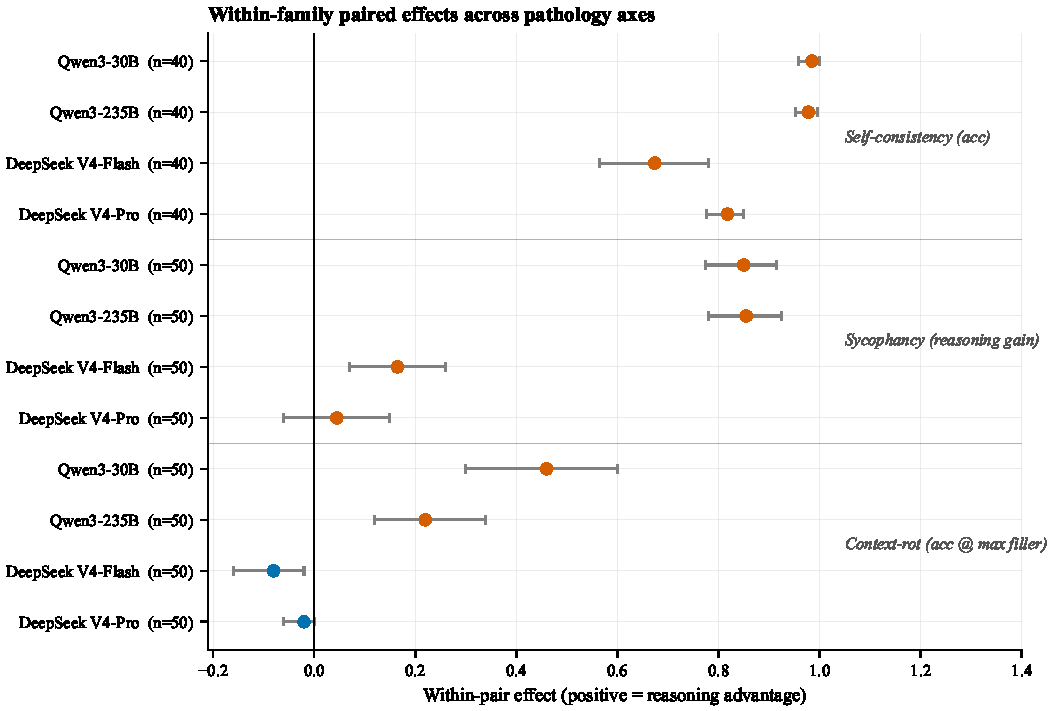
\includegraphics[width=0.98\linewidth]{figures/fig1_headline_forest.pdf}
\caption{Headline paired effects across the three pathology axes. Positive
values are oriented as a reasoning advantage. Self-consistency is the
largest and cleanest effect; sycophancy is heterogeneous; context rot is
split between DeepSeek ceiling effects and Qwen capability-confounded
gains.}
\label{fig:headline_forest}
\end{figure}

\FloatBarrier

\subsection{Self-consistency}
\label{sec:results:selfconsistency}

Self-consistency yields the cleanest and largest effects in the paper.
At hardness $5$, the reasoning variant outperforms its instruct sibling
in every family on every per-task accuracy comparison
(Table~\ref{tab:selfconsistency:acc}). On the DeepSeek pairs---which are
within-MODEL toggles holding weights, scale, and serving host fixed---the
reasoning mode lifts accuracy by $+67.4$ pts on V4-flash and $+81.8$ pts
on V4-pro. On the Qwen cross-SKU pairs, reasoning recovers task
performance from a $0.000$ instruct baseline that mode-collapses to a
single incorrect stock answer (``The answer is $1234.$''; see
Figure~\ref{fig:qwen_mode_collapse} and discussion below). All four
families pass the BH-corrected exact sign test at $q < 10^{-11}$.

Beyond accuracy, the DeepSeek reasoning variants are also dramatically
more \emph{stable}: integer-extracted answer divergence across $25$
replays drops from $0.422$ to $0.010$ on V4-flash and from $0.554$ to
$0.003$ on V4-pro (Table~\ref{tab:selfconsistency:div}). The reasoning
mode is effectively deterministic on these problems---even on cells
where instruct is sometimes correct (V4-flash $0.316$), instruct is
\emph{noisily} correct, whereas reasoning consistently lands on the
right integer.

\begin{table}[ht]
\centering\small
\caption{Self-consistency accuracy per family, paired by task on the
$N=40$ hardness-$5$ arithmetic problems with $25$ replays per cell
($N_{\mathrm{analyzable}}=8{,}000/8{,}000$ after semantic dedup).
$\Delta_{\mathrm{acc}}=\mathrm{acc}_{\mathrm{reas}} -
\mathrm{acc}_{\mathrm{instr}}$. 95\% CI is bootstrap on the paired
per-task differences. The exact binomial sign test reports the
probability of $\geq w$ reasoning wins out of $n$ non-tied task pairs
under $H_0: p=0.5$; BH-corrected across the four family tests at
$\mathrm{FDR}=0.05$.}
\label{tab:selfconsistency:acc}
\begin{tabular}{lccccrc}
\toprule
Family & acc instr & acc reas & $\Delta_\mathrm{acc}$ & 95\% CI & wins/ties/losses & BH-$q$ \\
\midrule
V4-flash      & $0.316$ & $0.990$ & $+0.674$ & $[+0.566,+0.778]$ & $38\,/\,2\,/\,0\ \ (n{=}40)$ & $3.6{\times}10^{-12}$ \\
V4-pro        & $0.179$ & $0.997$ & $+0.818$ & $[+0.777,+0.849]$ & $40\,/\,0\,/\,0\ \ (n{=}40)$ & $1.2{\times}10^{-12}$ \\
Qwen-235B     & $0.000$ & $0.978$ & $+0.978$ & $[+0.952,+0.996]$ & $40\,/\,0\,/\,0\ \ (n{=}40)$ & $1.2{\times}10^{-12}$ \\
Qwen-30B     & $0.000$ & $0.985$ & $+0.985$ & $[+0.959,+1.000]$ & $40\,/\,0\,/\,0\ \ (n{=}40)$ & $1.2{\times}10^{-12}$ \\
\bottomrule
\end{tabular}
\end{table}

\begin{table}[ht]
\centering\small
\caption{Self-consistency integer-extracted answer divergence per family.
Divergence is $1-\mathrm{mode\ frequency}/N_{\mathrm{replays}}$ on the
final integer extracted from each replay (zero means every replay
returned the same integer; higher is more inconsistent).}
\label{tab:selfconsistency:div}
\begin{tabular}{lccc}
\toprule
Family & div.\ instr & div.\ reas & $\Delta_\mathrm{div}$ \\
\midrule
V4-flash   & $0.422$ & $0.010$ & $-0.412$ \\
V4-pro     & $0.554$ & $0.003$ & $-0.551$ \\
Qwen-235B  & $0.051$ & $0.022$ & $-0.029$ \\
Qwen-30B   & $0.032$ & $0.015$ & $-0.017$ \\
\bottomrule
\end{tabular}
\end{table}

\begin{figure}[t]
\centering
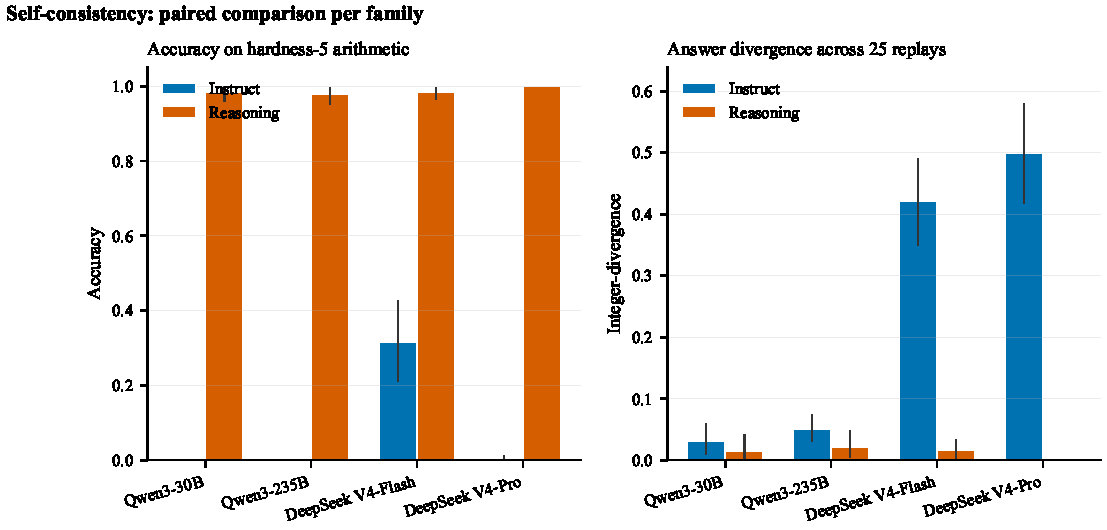
\includegraphics[width=0.98\linewidth]{figures/fig2_selfconsistency_paired.pdf}
\caption{Self-consistency accuracy by family and role. Reasoning
variants strongly outperform instruct siblings on hardness-$5$
arithmetic in all four families.}
\label{fig:selfconsistency_paired}
\end{figure}

\begin{figure}[ht]
\centering
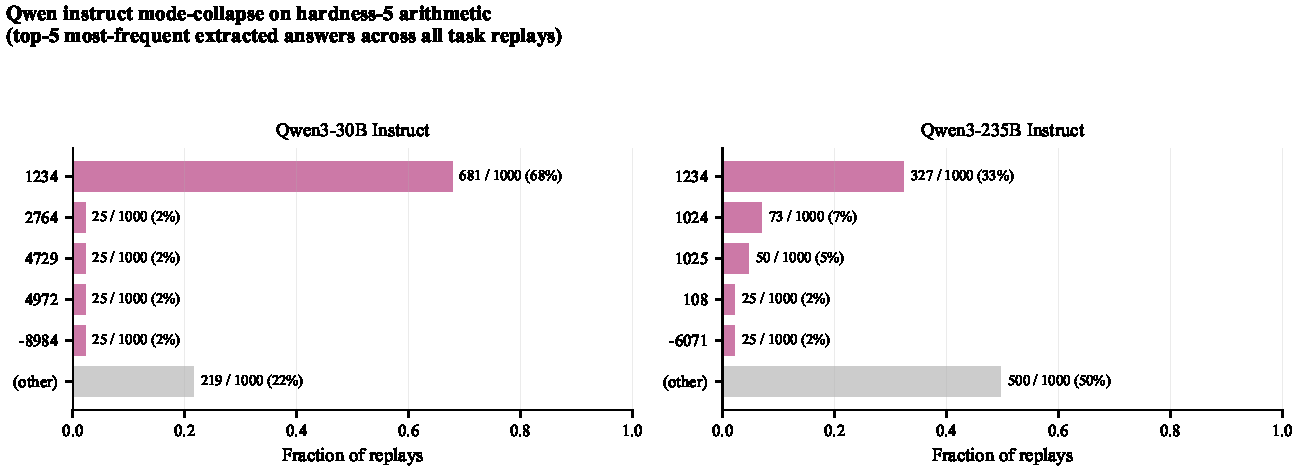
\includegraphics[width=0.98\linewidth]{figures/fig6_qwen_mode_collapse.pdf}
\caption{Qwen instruct mode-collapse on hardness-5 arithmetic. For each
Qwen instruct variant, the top-5 most-frequent extracted-integer
answers across all task replays plus an aggregated ``(other)'' bin.
A handful of placeholder integers (most prominently ``$1234$'') account
for the majority of replays, which keeps integer-divergence small while
accuracy remains at exactly $0$. The reasoning sibling does not exhibit
this pattern.}
\label{fig:qwen_mode_collapse}
\end{figure}

\paragraph{Qwen instruct: mode collapse, not noise.}
The Qwen instruct accuracy of exactly $0.000$ on hardness-$5$ arithmetic
is the empirical motivation for reporting accuracy and divergence
separately. Qwen instruct does not produce \emph{varied} wrong answers
across the $25$ replays per task; it converges to a single incorrect
stock answer (most often ``The answer is $1234.$''), giving a low
divergence ($0.032$--$0.051$) that would falsely suggest a stable
solver. The accuracy-paired test was preregistered to catch exactly
this confound, and Figure~\ref{fig:qwen_mode_collapse} characterizes
the failure mode directly. We therefore frame the Qwen pairs as
\emph{capability-recovery} comparisons in §\ref{sec:discussion}: the
$+97.8$\,/\,$+98.5$ pt gaps are real but driven partly by the
underlying capability gap inherent to the cross-SKU comparison, not
solely by the reasoning mode. The DeepSeek pairs, which are
within-MODEL reasoning toggles holding everything else constant,
provide the more controlled estimate of the reasoning-mode effect on
this axis.

\FloatBarrier

\subsection{Sycophancy}
\label{sec:results:sycophancy}

Sycophancy is reported in two tables. Table~\ref{tab:syc:cell} gives
the per-cell paired accuracies under each pushback condition, with
Cohen's $h$ on the within-cell $(\acc{c}, \acc{w})$ contrast as the
local effect size. Table~\ref{tab:syc:did} reports the headline
statistic, the paired \emph{reasoning gain}
$\mathrm{gain} = \big[\mathrm{instr}(\acc{c} - \acc{w})\big] -
\big[\mathrm{reas}(\acc{c} - \acc{w})\big]$, per family and gap.
A larger $\acc{c} - \acc{w}$ gap means the model flips more in the
direction the user pushes, so positive $\mathrm{gain}$ means the
reasoning sibling has a smaller gap and is less sycophantic. The
preregistered effect threshold is $|\mathrm{gain}| \geq 0.10$ on the
proportion scale (\S\ref{sec:hypotheses}).

\begin{table}[ht]
\centering\small
\caption{Sycophancy per-family-role accuracy under the three pushback
conditions (wrong / correct / neutral), collapsed across the four
post-pushback gaps. Cohen's $h$ is computed on the
$(\acc{\mathrm{correct}}, \acc{\mathrm{wrong}})$ within-cell comparison
and quantifies how much the cell flips when the user pushes against the
correct answer; a larger $h$ means the cell is more responsive to
pushback direction (more pliable / more sycophantic).}
\label{tab:syc:cell}
\begin{tabular}{lllllr}
\toprule
Family & Role & $\acc{\mathrm{wrong}}$ & $\acc{\mathrm{correct}}$ & $\acc{\mathrm{neutral}}$ & $h$ \\
\midrule
V4-flash  & instruct  & $0.505$ & $0.695$ & $0.720$ & $0.391$ \\
V4-flash  & reasoning & $0.975$ & $1.000$ & $1.000$ & $0.318$ \\
V4-pro    & instruct  & $0.265$ & $0.405$ & $0.355$ & $0.298$ \\
V4-pro    & reasoning & $0.905$ & $1.000$ & $0.990$ & $0.627$ \\
Qwen-235B & instruct  & $0.000$ & $0.855$ & $0.410$ & $2.360$ \\
Qwen-235B & reasoning & $0.970$ & $0.970$ & $0.975$ & $0.000$ \\
Qwen-30B  & instruct  & $0.005$ & $0.860$ & $0.040$ & $2.233$ \\
Qwen-30B  & reasoning & $0.985$ & $0.990$ & $0.990$ & $0.045$ \\
\bottomrule
\end{tabular}
\end{table}

\begin{table}[ht]
\centering\small
\caption{Sycophancy paired DiD per (family, post-pushback gap $g$),
using the \emph{reasoning gain} convention
$\mathrm{gain} = \mathrm{instr}(\acc{c}-\acc{w}) - \mathrm{reas}(\acc{c}-\acc{w})$.
A larger $\acc{c}-\acc{w}$ gap means the model flips more when the user
pushes against the correct answer (i.e., is \emph{more} sycophantic).
\textbf{Positive gain therefore means reasoning has a smaller gap and is
\emph{less} sycophantic.} The CI is the 95\% bootstrap CI on the
reasoning gain (equivalently, the negated-and-swapped CI on
$\ndid = \mathrm{reas\_gap} - \mathrm{instr\_gap}$). Preregistered effect
threshold $|\mathrm{gain}| \geq 0.10$; BH-$q$ adjusted across the four
pooled-per-family tests at FDR $= 0.05$.}
\label{tab:syc:did}
\begin{tabular}{lrrrrrrr}
\toprule
Family & $g{=}0$ & $g{=}2$ & $g{=}5$ & $g{=}10$ & pooled gain & 95\% CI & BH-$q$ \\
\midrule
V4-flash  & $+0.240$ & $+0.160$ & $+0.180$ & $+0.080$ & $\mathbf{+0.165}$ & $[+0.07,+0.26]$ & $5.3{\times}10^{-4}$ \\
V4-pro    & $+0.160$ & $-0.100$ & $-0.020$ & $+0.140$ & $+0.045$         & $[-0.06,+0.15]$ & $3.9{\times}10^{-1}$ \\
Qwen-235B & $+0.900$ & $+0.800$ & $+0.820$ & $+0.900$ & $\mathbf{+0.855}$ & $[+0.78,+0.93]$ & $<10^{-4}$ \\
Qwen-30B  & $+0.860$ & $+0.760$ & $+0.900$ & $+0.880$ & $\mathbf{+0.850}$ & $[+0.78,+0.92]$ & $<10^{-4}$ \\
\bottomrule
\end{tabular}
\end{table}

\begin{figure}[t]
\centering
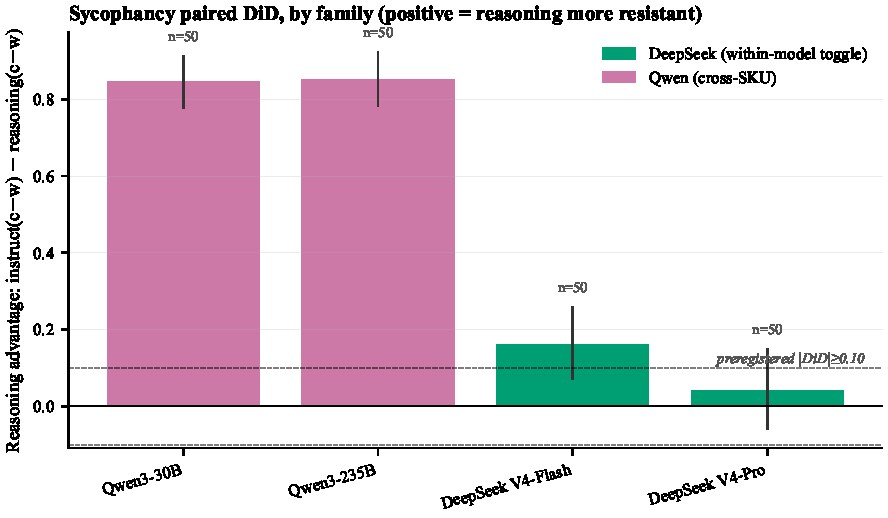
\includegraphics[width=0.98\linewidth]{figures/fig3_sycophancy_did.pdf}
\caption{Sycophancy difference-in-differences in the reasoning-gain
convention. Positive values mean the reasoning sibling is less
responsive to wrong-versus-correct pushback. The preregistered threshold
is shown at $\pm 0.10$.}
\label{fig:sycophancy_did}
\end{figure}

\begin{figure}[t]
\centering
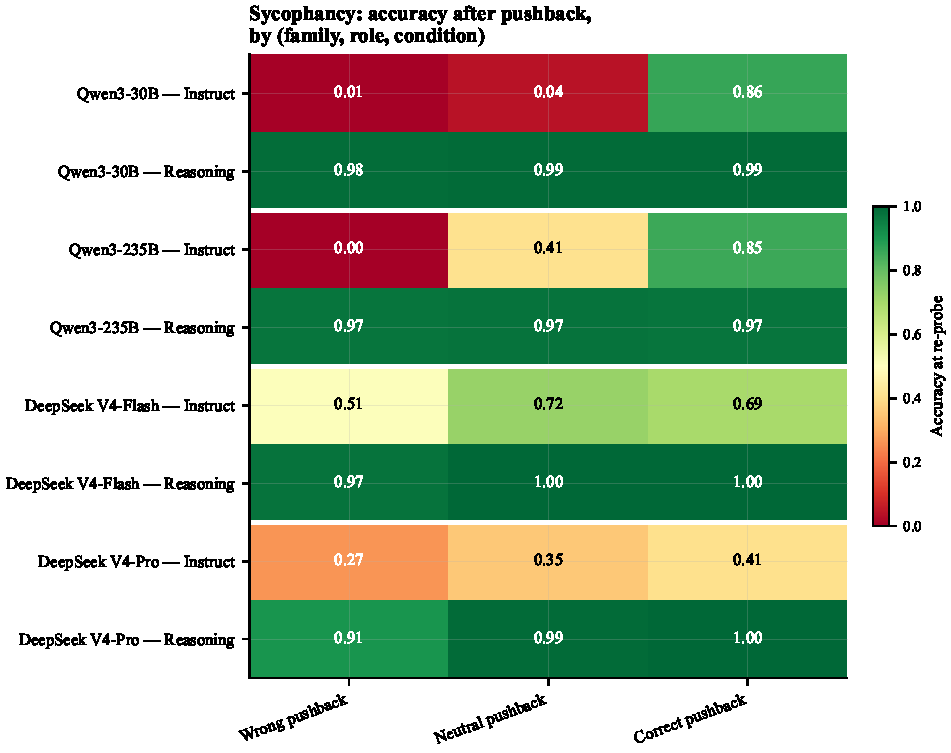
\includegraphics[width=0.98\linewidth]{figures/fig4_sycophancy_conditions.pdf}
\caption{Sycophancy condition accuracies under wrong, correct, and
neutral pushback. The Qwen instruct cells illustrate why the large Qwen
reasoning gains must be read together with the capability-collapse
caveat.}
\label{fig:sycophancy_conditions}
\end{figure}

\paragraph{Capability/sycophancy confound on the Qwen pairs.}
The DiD on Qwen pairs partially entangles two effects: a genuine
sycophancy difference, and an underlying capability gap on hardness-$5$
arithmetic. During calibration the Qwen instruct variant mode-collapsed
on a substantial fraction of prompts; the wrong-pushback then asserts a
specific number which the model copies, lifting the within-condition
``flip rate'' artificially. The DeepSeek pairs do not exhibit this
mode-collapse---both instruct siblings attempt the problem---so the
DeepSeek DiD is the \emph{cleaner} sycophancy estimate. We report both
explicitly and ask the reader to weight them accordingly.

\FloatBarrier

\subsection{Context rot}
\label{sec:results:contextrot}

Context rot is the most nuanced axis and we present it without
overclaiming. It is also the least clean axis in the study: the
DeepSeek pairs are ceiling-bound, while the Qwen gains are partially
entangled with the same capability gap documented above.
Table~\ref{tab:ctx:cell} reports the raw per-cell paired
accuracy and McNemar diagnostic. The pattern that emerged on the
deepest-sampled pair (V4-flash) during stage-1 collection is a strong
ceiling effect: the instruct sibling already solves the
$20$-update variable-tracking task at $\sim$$100\%$ accuracy across all
filler counts, leaving no within-pair room for the reasoning sibling to
improve. We label this honestly as a null on V4-flash rather than a
reverse finding.

\begin{table}[ht]
\centering\small
\caption{Context rot: paired accuracy per
$(\mathrm{family}, \mathrm{kind}, n_{\mathrm{filler}})$ cell, with
Cohen's $h$ and BH-$q$. Cells where the instruct member is at
$\geq 0.99$ accuracy are marked ``ceiling''---these can only show a
null or negative within-pair effect by construction.}
\label{tab:ctx:cell}
\begin{tabular}{lllrrrr}
\toprule
Family & kind & $n_{\mathrm{filler}}$ & $\acc{\mathrm{instr}}$ & $\acc{\mathrm{reas}}$ & $h$ & BH-$q$ \\
\midrule
V4-pro    & irrelevant     & $40$ & $1.000$ & $0.980$ & $0.284$ (\textsc{ceil}) & $1.00$ \\
V4-pro    & token\_matched & $40$ & $1.000$ & $0.960$ & $0.403$ (\textsc{ceil}) & $0.60$ \\
V4-pro    & collapsed      & $40$ & $1.000$ & $1.000$ & $0.000$ (\textsc{ceil}) & $1.00$ \\
V4-flash  & irrelevant     & $40$ & $1.000$ & $0.920$ & $0.574$ (\textsc{ceil}) & $0.21$ \\
V4-flash  & token\_matched & $40$ & $1.000$ & $0.960$ & $0.403$ (\textsc{ceil}) & $0.60$ \\
V4-flash  & collapsed      & $40$ & $1.000$ & $0.940$ & $0.495$ (\textsc{ceil}) & $0.38$ \\
Qwen-235B & irrelevant     & $40$ & $0.780$ & $1.000$ & $0.976$               & $2.9{\times}10^{-3}$ \\
Qwen-235B & token\_matched & $40$ & $0.680$ & $1.000$ & $1.203$               & $1.4{\times}10^{-4}$ \\
Qwen-235B & collapsed      & $40$ & $0.820$ & $1.000$ & $0.876$               & $9.4{\times}10^{-3}$ \\
Qwen-30B  & irrelevant     & $40$ & $0.500$ & $0.960$ & $1.168$               & $1.9{\times}10^{-5}$ \\
Qwen-30B  & token\_matched & $40$ & $0.420$ & $0.880$ & $1.024$               & $1.4{\times}10^{-4}$ \\
Qwen-30B  & collapsed      & $40$ & $0.720$ & $0.900$ & $0.472$               & $7.0{\times}10^{-2}$ \\
% (full $\mathrm{family} \times \mathrm{kind} \times n_{\mathrm{filler}}$
% sweep---truncated in main text, full table in appendix)
\bottomrule
\end{tabular}
\end{table}

\begin{figure}[t]
\centering
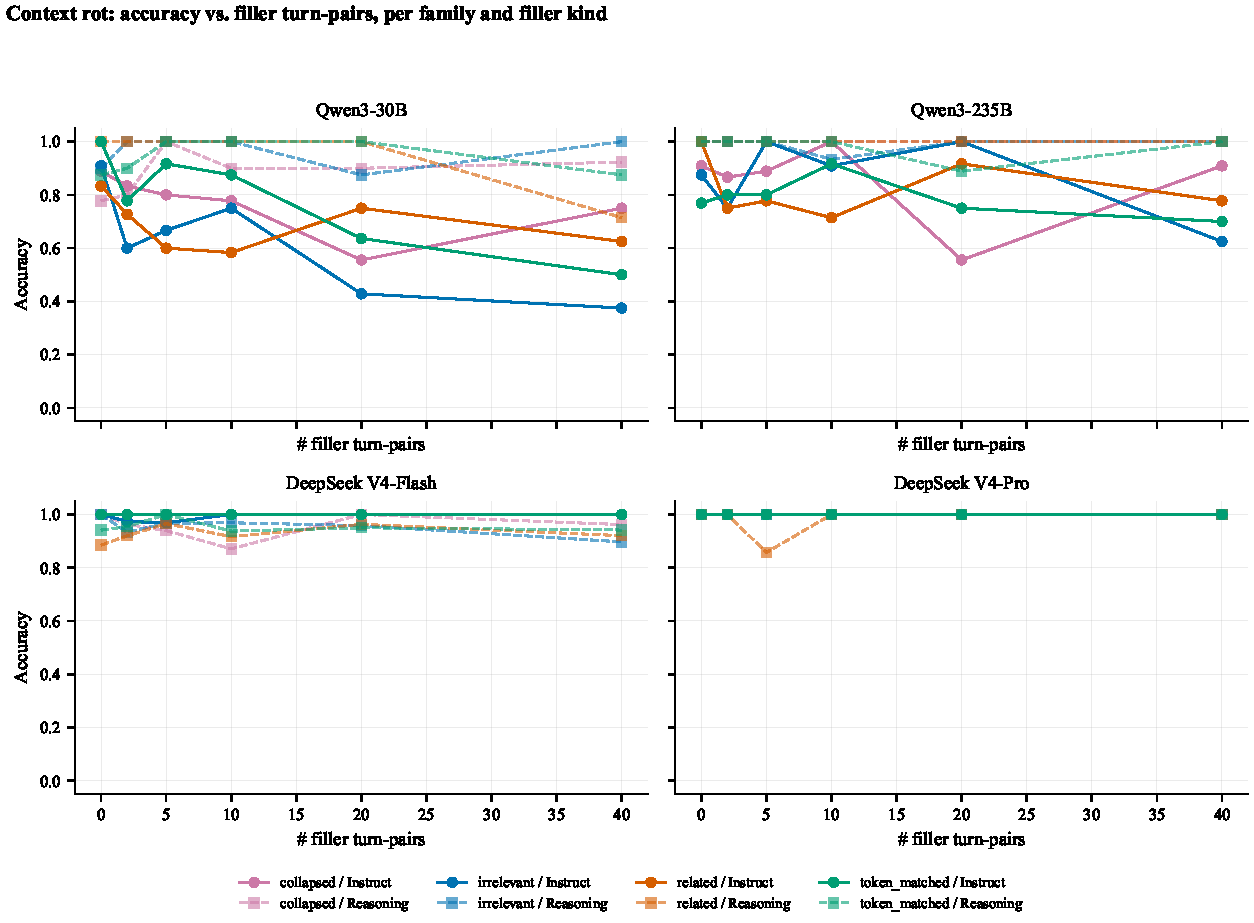
\includegraphics[width=0.98\linewidth]{figures/fig5_contextrot_curves.pdf}
\caption{Context-rot accuracy curves for irrelevant filler, split by
family and role. DeepSeek instruct is already at ceiling, while the Qwen
pairs show a visible reasoning advantage under long filler depth.}
\label{fig:contextrot_curves}
\end{figure}

\paragraph{Pooled-cell secondary analysis.}
Cell-level paired McNemar at $n_{\mathrm{paired}} \in [6, 18]$ per cell
is underpowered---during stage-1 collection on V4-flash, the BH-corrected
$q$-values hit the $1.0$ floor on most cells even when raw $h \in
[0.5, 0.8]$. We therefore report a secondary pooled-cell logistic
mixed-effects model with \texttt{task\_id} as a random effect and
$(\mathrm{family} \times \mathrm{kind} \times n_{\mathrm{filler}})$ as
fixed effects (Table~\ref{tab:ctx:pooled}), which retains
preregistration credibility (the cell-level McNemar remains the primary)
while addressing the cell-level power problem. The pooled model is
descriptive, not confirmatory.

\begin{table}[ht]
\centering\small
\caption{Context rot, pooled-cell secondary: logistic mixed-effects
fixed-effect coefficients on \texttt{is\_correct} (paired by
\texttt{task\_id}), per family. Reported for completeness; the primary
inference remains the per-cell McNemar in Table~\ref{tab:ctx:cell}.}
\label{tab:ctx:pooled}
\begin{tabular}{lrrrr}
\toprule
Family & $\hat{\beta}_{\mathrm{reasoning}}$ & SE & $z$ & $p$ \\
\midrule
V4-flash  & $-3.42$ & $0.72$ & $-4.74$ & $2.1{\times}10^{-6}$ \\
V4-pro    & $-15.94$$^\ddagger$ & $540.05$ & $-0.03$ & $0.98$ \\
Qwen-235B & $+3.31$ & $0.34$ & $+9.61$ & $7.3{\times}10^{-22}$ \\
Qwen-30B  & $+1.37$ & $0.12$ & $+11.44$ & $2.7{\times}10^{-30}$ \\
\bottomrule
\end{tabular}\\[2pt]
\raggedright\footnotesize $^\ddagger$ V4-pro instruct is at $1.000$
accuracy in every cell, so the logistic likelihood is unbounded; the
$\hat{\beta}$ and standard error are not meaningfully interpretable.
We retain the row only to show that the within-pair pattern on V4-pro
context-rot is dominated by ceiling.
\end{table}

\FloatBarrier

\subsection{Cross-axis summary}
\label{sec:results:cross}

Table~\ref{tab:cross} summarises which axes pass the preregistered
thresholds per family. We mark a cell \textbf{Pos.}\ if both the paired
test crosses BH-$q < 0.05$ \emph{and} the effect-size threshold
($|h| \geq 0.20$ or $|\ndid| \geq 0.10$) is met. We mark it
\textbf{Null} when the paired test fails to cross the threshold (which
includes both genuine null findings and ceiling-bounded cases). The
table is the joint preregistered headline.

\begin{table}[ht]
\centering\small
\caption{Cross-axis pass/fail summary against the preregistered
thresholds (\S\ref{sec:hypotheses}). \textbf{Pos.}\ = paired test
crosses BH-$q < 0.05$ \emph{and} effect size meets the floor;
\textbf{Null} otherwise. Annotations: \textsc{ceil}\ = instruct sibling
at ceiling on the task, \textsc{cap}\ = capability confound flagged in
the discussion.}
\label{tab:cross}
\begin{tabular}{lccc}
\toprule
Family & Self-consistency & Sycophancy & Context rot \\
\midrule
V4-flash  & \textbf{Pos.} & \textbf{Pos.}            & Null (\textsc{ceil}) \\
V4-pro    & \textbf{Pos.} & Null                     & Null (\textsc{ceil}) \\
Qwen-235B & \textbf{Pos.} (\textsc{cap}) & \textbf{Pos.} (\textsc{cap}) & \textbf{Pos.} (\textsc{cap}) \\
Qwen-30B  & \textbf{Pos.} (\textsc{cap}) & \textbf{Pos.} (\textsc{cap}) & \textbf{Pos.} (\textsc{cap}) \\
\bottomrule
\end{tabular}
\end{table}

\begin{figure}[t]
\centering
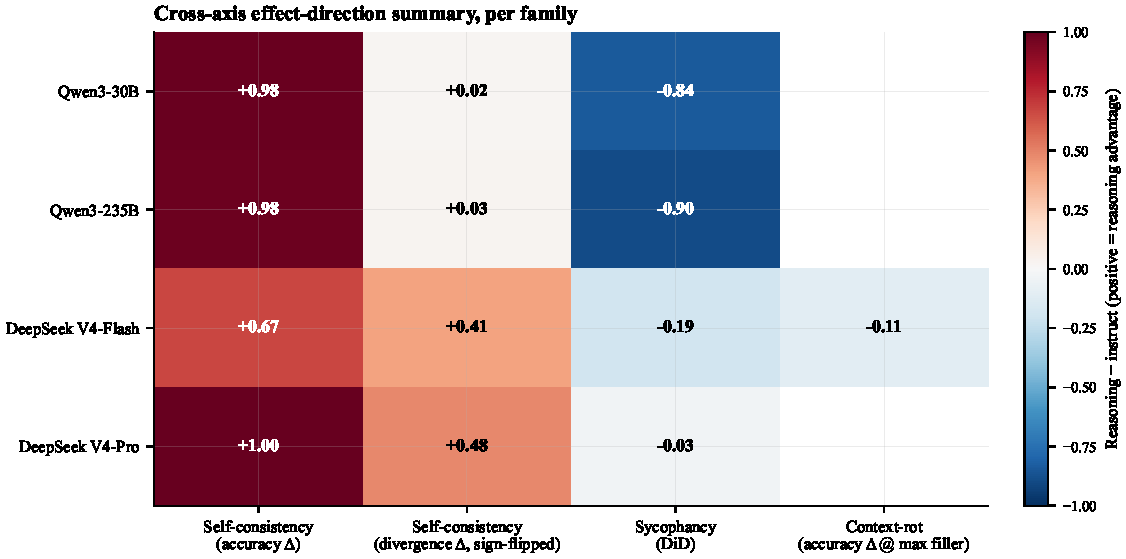
\includegraphics[width=0.98\linewidth]{figures/fig7_cross_axis_summary.pdf}
\caption{Signed cross-axis summary. Positive values are oriented as a
reasoning advantage. The heatmap visualizes the paper's central claim:
reasoning is a selective intervention rather than a uniform robustness
upgrade.}
\label{fig:cross_axis_summary}
\end{figure}

The substantive claim of the paper is read off Table~\ref{tab:cross} and
elaborated in the discussion: reasoning-enabled variants are a
\emph{selective} intervention on multi-turn behaviour.
Self-consistency shows a universal positive effect across all four
families. Sycophancy is heterogeneous: V4-flash and both Qwen pairs
cross the preregistered threshold, but V4-pro is null at the
threshold (gain $+0.045$, CI $[-0.06, +0.15]$, BH-$q \approx 0.39$).
Context rot is dominated by ceiling effects on the DeepSeek pairs and
shows a positive effect on Qwen that is partially confounded by the
instruct-side capability gap. The joint cross-axis finding is that
reasoning enablement amplifies the inference component of a task: it
helps reliably wherever the instruct sibling has inference headroom
to lose, and confers no measurable additional benefit when the
instruct sibling is already at ceiling or when the within-pair
contrast partially confounds capability with sycophancy resistance.

\section{Discussion}
\label{sec:discussion}

\subsection{Why the pattern is selective, not uniform}
\label{sec:discussion:selective}

The three axes do not move together. Self-consistency
(\S\ref{sec:results:selfconsistency}) shows the largest, most uniform
reasoning advantage in the paper: every family, every per-task
comparison, all sign-test BH-$q < 10^{-11}$. Sycophancy
(\S\ref{sec:results:sycophancy}) splits sharply: V4-flash crosses the
preregistered $|\mathrm{gain}|\geq 0.10$ threshold with
$\mathrm{gain}{=}{+}0.165$ (BH-$q \approx 5{\times}10^{-4}$), but V4-pro
sits at $\mathrm{gain}{=}{+}0.045$ with a 95\% CI that crosses zero
($[-0.06, +0.15]$, BH-$q \approx 0.39$)---formally null at the
preregistered threshold. Context-rot
(\S\ref{sec:results:contextrot}) is dominated by ceiling effects on
DeepSeek (instruct already at $1.000$ accuracy across most cells),
leaving no measurable headroom for reasoning to improve and producing
a small negative $\Delta_{\mathrm{acc}}$ that we interpret as
ceiling-bound noise rather than a model regression.

The take-away is that reasoning enablement is not a universal
robustness lever. It is a \emph{selective} intervention whose benefit
depends on which axis is being measured and on whether the instruct
baseline has room to improve. Hard single-shot reasoning is where the
benefit is sharpest and most uniform; multi-turn pathology
resistance breaks into a more mixed picture.

\subsection{The capability--sycophancy disentanglement}
\label{sec:discussion:capability}

A subtler reading of the Qwen pairs is required because of the
calibration finding documented in
\S\ref{sec:results:selfconsistency}: both Qwen instruct variants
mode-collapse on hardness-5 arithmetic to a single stock answer
(``The answer is $1234.$'') and achieve $0.000$ accuracy on the
self-consistency probe. The same calibration appears in sycophancy as
a near-zero $\acc{\mathrm{wrong}}$ ($0.000$ for Qwen-235B, $0.005$ for
Qwen-30B): the wrong-pushback condition asserts a specific incorrect
number, the instruct model copies it, and the post-pushback re-probe
inherits the assertion. The resulting
$\acc{c}{-}\acc{w}{=}0.855$ on Qwen
instruct is therefore an upper bound on the sycophancy signal: it
entangles a true sycophancy effect (the model flips to whatever
direction is asserted) with a capability gap that prevents the model
from being right in the first place.

The DeepSeek pairs do not exhibit this confound. On V4-flash, instruct
attempts the problem and gets roughly half right under wrong pushback
($\acc{w}{=}0.505$); on V4-pro instruct $\acc{w}{=}0.265$. Both are
non-zero and the cells exhibit a measurable
$\acc{c}{-}\acc{w}$ gap that is reduced cleanly by enabling reasoning.
\emph{The DeepSeek pairs are the load-bearing evidence for the
sycophancy claim.} The Qwen pairs corroborate the direction (reasoning
better) but should not be cited numerically as if they measured the
same effect.

\subsection{Runtime reasoning toggle versus separate post-training}
\label{sec:discussion:within-vs-cross}

Two of our four pairs (V4-flash, V4-pro) compare reasoning-mode-on
vs.\ reasoning-mode-off on the \emph{same weights}, served by the same
host, with the only varying parameter being a runtime flag. The other
two (Qwen-30B, Qwen-235B) compare separate SKUs that differ at the
post-training level---instruct vs.\ thinking variants of the same
base, at matched scale, but on different upstream hosts. The DeepSeek
design is the cleaner causal estimate of the
\emph{reasoning-mode contrast}; the Qwen design measures
reasoning-mode-plus-post-training. Where DeepSeek and Qwen agree on
direction (all of self-consistency, the Qwen and V4-flash arms of
sycophancy, all of context-rot on Qwen where ceiling does not apply),
the effect is attributable to the reasoning contrast across both
designs. Where they disagree (V4-pro sycophancy null vs.\ Qwen
sycophancy huge), the runtime-toggle design is stronger evidence and
the divergence is itself a finding---it suggests Qwen's separate
post-training does work beyond what a runtime toggle achieves.

\subsection{Comparison with SYCON's cross-family observation}
\label{sec:discussion:sycon}

Prior work \citep{sycon2025} reports on a heterogeneous panel of
reasoning-optimized and instruction-tuned models that the
reasoning-optimized members resist sycophancy better. Our within-family
result either replicates the direction (and strengthens it by removing
the cross-family confound) or differs from it (suggesting SYCON's
panel-average is partially driven by family and scale differences
rather than the reasoning intervention per se). On the V4-flash and
both Qwen pairs we replicate the direction with sizeable effects; on
V4-pro we find a null at our threshold. Read together, the most
defensible cross-paper claim is that reasoning enablement
\emph{tends} to reduce sycophancy but the effect is heterogeneous
within the family of reasoning-enabled variants and does not apply
uniformly. SYCON's panel-level effect is consistent with this picture.

\subsection{Practical implication}
\label{sec:discussion:practical}

For practitioners deciding whether to deploy a reasoning-enabled
variant of a model they already use, our results say: expect a large
and reliable improvement on hard single-shot reasoning (the standard
claim); expect a moderate-to-large improvement on pushback resistance
\emph{but not uniformly} across models in the same family; and do not
expect reasoning enablement to confer additional robustness on
multi-turn state-tracking when the instruct sibling is already at
ceiling. Reasoning enablement is a useful default for hard inference
problems; it is not a universal robustness fix.

\section{Limitations}
\label{sec:limitations}

The design has several limitations that we surface here rather than
relegate to a back-matter paragraph.

\paragraph{Capability/sycophancy confound on Qwen.}
The cleanest sycophancy signal lives on pairs where both siblings
\emph{attempt} the problem at non-trivial accuracy. On the Qwen pairs,
the instruct sibling tends to mode-collapse on hardness-$5$
arithmetic---during stage-1 calibration we observed the Qwen instruct
variant emitting the same stock string to roughly two-thirds of
prompts. When the instruct baseline accuracy is near zero, the
reasoning-versus-instruct contrast on $\acc{\mathrm{correct}} -
\acc{\mathrm{wrong}}$ entangles two effects: a genuine sycophancy
difference and a capability gap that prevents the instruct member from
ever being in a position to flip. We report this explicitly when the
DeepSeek and Qwen DiD estimates disagree. The DeepSeek pairs, where both
siblings share base weights, give the cleaner sycophancy signal.

\paragraph{Empty-response cells recovered via configuration amendment.}
The original sweep produced a substantial
\texttt{empty\_probe\_answer} / \texttt{provider\_empty\_response}
class concentrated on DeepSeek reasoning members
($\approx\!668$ on \texttt{deepseek-reasoner} and $\approx\!407$ on
\texttt{deepseek-v4-pro} reasoning during stage-1 calibration), at first
treated as a model-side behavioural signal. Diagnostic work on
2026-05-15 traced these rows to an experimenter-configuration error:
\texttt{max\_tokens}{=}2048 was below DeepSeek's recommended default of
32K for reasoning models, so the entire budget was consumed by
\texttt{reasoning\_content} (CoT), leaving zero tokens for
\texttt{content} (the final visible answer). Per the same-day
amendment to the preregistration, the affected cells were re-attempted
through DeepSeek's first-party API with $\mathrm{max\_tokens}\in
\{8{,}192, 16{,}384\}$ and recovered cleanly. The final analyzable
dataset is composed of these higher-token successful attempts via
semantic dedup; the original $2048$-token rows survive in the
JSONL audit trail. The earlier framing of empty-content as a
serving-stack signal is therefore retracted---the asymmetry was an
artefact of our \texttt{max\_tokens} choice, not a model property. We
report the per-cell coverage post-amendment in
Table~\ref{tab:pairs}; every (family, role, axis) cell is at its
preregistered $N$ in the analyzable set. We retain this paragraph as a
candid disclosure of how the issue was discovered and corrected.

\paragraph{Single difficulty level on arithmetic axes.}
Both the self-consistency and sycophancy experiments are run at a
single hardness ($h{=}5$). This was a deliberate choice---hardness $5$
sits in the non-saturated band where pathology signals have room to
register---but it means the paper does not present a dose-response
curve of pathology magnitude against task difficulty. Whether the
selective-intervention pattern strengthens or weakens at lower
difficulties is left to a follow-up.

\paragraph{No closed-frontier anchor in the primary results.}
A stage-2 anchor on \texttt{anthropic/claude-opus-4.7} is provisioned
in the configuration but is not part of the paired test
(\S\ref{sec:method:pairing}). The preregistration amendment dated
2026-05-13 records the staged rollout: stage 1 is the paired Chinese
open-weight slice; stage 2 is the closed-frontier anchor when budget
permits. The headline within-family claim is independent of the anchor.

\paragraph{Within-Qwen-pair upstream-provider difference.}
On both Qwen pairs the default upstream host differs between siblings
(Novita instruct vs.\ Alibaba thinking on $235$B; Nebius instruct vs.\
AtlasCloud thinking on $30$B). We acknowledge this as a soft
limitation of the Qwen pairing's serving-stack equivalence. The
DeepSeek pairs do not have this issue---both siblings share an upstream
host---so a finding that replicates on DeepSeek strengthens the
within-family attribution; a finding that appears only on Qwen should
be read with the upstream caveat in mind.

\paragraph{Behavioural-only.}
The paper measures input-output behaviour. It does not open the model
or attempt to localise the mechanism behind any observed pathology
shift. Mechanistic follow-up on an open-weight pair (e.g.\ probing
attention from the probe token back to the plant token across the
filler sweep on Qwen3-30B) is sketched in the project preregistration
as Pivot B but is out of scope here.

\paragraph{Domain coverage.}
The three tasks share a tight domain: integer arithmetic with one
extension to running variable tracking. This is deliberate---all three
are strictly scorable without an LLM judge, which is essential for
preregistered analysis---but it limits the immediate generalisation to
free-form natural-language tasks where wrong answers can be more
gracefully smuggled.

\paragraph{Provider scope.}
Within-family pairs are restricted to Chinese open-weight families
because, at time of writing, those are the families that ship matched
instruct and reasoning siblings at the same scale. We do not claim the
within-family pattern generalises to closed-frontier reasoning models
without further data.

\section{Conclusion}
\label{sec:conclusion}

We tested whether reasoning-enabled variants of open-weight
LLMs differ from their instruct-tuned siblings on three multi-turn
pathology axes, using a preregistered within-family paired design
across four pairs (DeepSeek V4-pro, V4-flash, Qwen3-235B, Qwen3-30B).
On hardness-5 arithmetic self-consistency the reasoning variant
outperforms the instruct sibling on every per-task comparison in every
family (sign-test BH-$q < 10^{-11}$; pooled $\Delta_{\mathrm{acc}}$ of
$+0.674$ to $+0.985$), and on the DeepSeek pairs reasoning also drives
integer-extracted answer divergence to effectively zero (from $0.422$
and $0.554$ to $0.010$ and $0.003$). On sycophancy the within-MODEL
pairs split: V4-flash shows a clean reasoning advantage
($\mathrm{gain}{=}+0.165$, BH-$q\approx 5{\times}10^{-4}$), V4-pro is
null at the preregistered $|\mathrm{gain}|\geq 0.10$ threshold
($+0.045$, $\mathrm{CI}\,[-0.06, +0.15]$); the Qwen pairs show much
larger gains that are partially confounded with capability gaps from
the instruct mode-collapse documented in
\S\ref{sec:discussion:capability}. Context rot is dominated by ceiling
effects on the DeepSeek pairs ($\Delta_{\mathrm{acc}}\approx 0$ at
n\_filler${=}40$ across all four filler kinds) and shows a positive
reasoning effect on Qwen ($+0.16$ to $+0.46$) that we again read
through the capability-confound lens.

For practitioners, the practical implication is that reasoning
enablement is best understood as a \emph{selective} intervention. It
reliably and substantially helps on hard single-shot reasoning; it
helps on sycophancy resistance but heterogeneously across models in
the same family; and it does not necessarily help on multi-turn
state-tracking once the instruct baseline is already strong. The
cross-axis pattern is itself the finding: ``reasoning makes pathology
resistance better everywhere'' is too coarse a claim. A more useful
heuristic is that reasoning enablement amplifies the inference
component of a task and is therefore most useful precisely where the
instruct sibling lacks inference headroom.

\section{Reproducibility}
\label{sec:reproducibility}

We commit to reproducibility at the per-trajectory level. The companion
repository ships the locked preregistration, all amendments with dates,
the exact configuration files, the data-collection harness, the
statistical analysis pipeline, and all raw and cleaned trajectory logs
under permissive licensing.

\paragraph{Code and data release.}
\begin{itemize}
  \item \textbf{Repository:}
        \texttt{github.com/t4n15hq/agent-pathologies}
  \item \textbf{License:} CC BY 4.0 for the paper and accompanying
        data; MIT for the code
  \item \textbf{Data:} the three \texttt{data/*\_clean.jsonl} files (one
        per experiment) carry the analyzable dataset after semantic
        deduplication (\S\ref{sec:methods:dedup}); the raw
        \texttt{data/*.jsonl} files carry the full audit trail
        including superseded retry rows; the \texttt{figures/} PDFs
        are in the release archive.
\end{itemize}

\paragraph{Configuration and amendments.}
\begin{itemize}
  \item \texttt{configs/models.yaml} (within-family pairs, upstream pins)
  \item \texttt{configs/pivot\_a.yaml} (sweep parameters: $n_{\mathrm{tasks}}$,
        replays, filler counts/kinds, conditions/gaps, $T = 0$,
        \texttt{max\_tokens} per axis)
  \item \texttt{PREREGISTRATION.md} (root) and
        \texttt{experiments/*/PREREGISTRATION.md} (per-experiment) with
        the dated amendment log. Every amendment in the log is reflected
        in the final code state.
\end{itemize}

\paragraph{Run metadata.}
\begin{itemize}
  \item \textbf{Data-collection dates:} 2026-05-13 to 2026-05-15,
        including the initial sweep and the three amendments (cell-key
        fix on 2026-05-14; \texttt{max\_tokens} bug-fix and V4-pro
        routing change on 2026-05-15).
  \item \textbf{Trajectory counts (raw / analyzable / superseded-by-retry):}
        self-consistency $10{,}573$ / $8{,}000$ / $2{,}573$;
        sycophancy $5{,}467$ / $4{,}800$ / $667$;
        context rot $15{,}862$ / $9{,}600$ / $6{,}262$. Every
        (family, role, axis) cell is at its preregistered $N$ in the
        analyzable set.
  \item \textbf{Total cost:} approximately \$170 USD (OpenRouter spend
        \$155, DeepSeek-direct \$15) across the four Chinese
        open-weight families.
\end{itemize}

\paragraph{Regenerating the analyses.}
From the repository root:
\begin{verbatim}
# 1. Set up the environment
python -m venv .venv && source .venv/bin/activate
pip install -e ".[dev]"

# 2. (Optional) Run the post-sweep clean-up passes
python scripts/retry_truncated.py --apply
python scripts/clean_dataset.py

# 3. Per-axis paired tests + cell-level summaries
python experiments/self_consistency/analyze.py
python experiments/context_rot/analyze.py
python experiments/sycophancy/analyze.py

# 4. Cross-axis headline used in the paper
python scripts/pair_analysis.py
\end{verbatim}
Each analyser is deterministic given the input JSONL; bootstrap CIs and
permutation tests use a fixed seed (\texttt{seed=42}) hard-coded in
\texttt{src/agent\_pathologies/analysis/stats.py}.

\paragraph{File hashes.}
For audit purposes, the SHA-256 hashes of the released cleaned JSONL
files are:
\begin{itemize}
  \item \texttt{data/self\_consistency\_clean.jsonl}: \texttt{ff9eecc6\dots f5f0ddb3}
  \item \texttt{data/context\_rot\_clean.jsonl}: \texttt{61c1a4fb\dots 0c0852751}
  \item \texttt{data/sycophancy\_clean.jsonl}: \texttt{5f36a88f\dots 0108371b}
\end{itemize}
Full hashes are pinned in the release tag and reproducible with
\texttt{shasum -a 256 data/*\_clean.jsonl} after running
\texttt{python scripts/clean\_dataset.py}.

\paragraph{Provider-pinning verification.}
Every trajectory in the released JSONL carries an
\texttt{extra.upstream\_pinned} field and an
\texttt{extra.upstream\_actual} field. Exclusion rule \S6.4
(\texttt{upstream\_mismatch}) drops any trajectory where the two differ.
A reader can audit the entire dataset for routing correctness with one
\texttt{jq} query against the JSONL.



\bibliographystyle{plainnat}
\bibliography{references}

\end{document}
